\documentclass[10pt]{beamer}
\usetheme{CambridgeUS}
\usecolortheme{beaver}
\usepackage[utf8]{inputenc}
\usepackage{amsmath,amssymb}
\usepackage{graphicx}
\usepackage{booktabs}
\usepackage{hyperref}
\usepackage{listings}
\usepackage[dvipsnames]{xcolor}

\graphicspath{{figures/}}

\title{Predicting Insurance Costs: Analysis and Insights}
\author{SDS Mini-Datathon Team}
\institute[NUS]{National University of Singapore}
\date{\today}

\begin{document}

\begin{frame}
\titlepage
\end{frame}

\begin{frame}{Problem Framing \& Objective}
\begin{itemize}
\item \textbf{Challenge}: Predict medical insurance charges using demographic and lifestyle data
\item \textbf{Goal}: Build accurate regression models and identify key cost drivers
\item \textbf{Importance}: Fair pricing, risk assessment, healthcare insights
\item \textbf{Dataset}: 1,338 records with age, sex, BMI, children, smoker, region, charges
\item \textbf{Equity Context}: Recent studies highlight insurance pricing inequities
  \begin{itemize}
  \item NAIC Special Committee on Race and Insurance
  \item Concerns over credit scoring as proxy discriminator
  \item Our analysis ensures fairness through statistical testing
  \end{itemize}
\end{itemize}
\end{frame}

\begin{frame}{Dataset and Features}
\small
\begin{table}[h]
\centering
\begin{tabular}{@{}lll@{}}
\toprule
Feature & Type & Notes \\
\midrule
age & integer & years \\
sex & categorical & male/female (encoded) \\
bmi & float & body mass index \\
children & integer & number of dependents \\
smoker & categorical & yes/no (encoded) \\
region & categorical & NE/NW/SE/SW (encoded) \\
\midrule
\textit{Engineered} & & \\
bmi\_category & categorical & underweight/normal/overweight/obese \\
age\_group & categorical & young/middle/senior \\
\bottomrule
\end{tabular}
\caption{Dataset schema and engineered features}
\end{table}
\end{frame}

\begin{frame}{Exploratory Data Analysis}
\begin{itemize}
\item Data quality: No missing values, clean dataset
\item Key statistics: Charges range \$1,122--\$63,771 (mean \$13,270)
\item Distribution: Right-skewed charges, normal BMI/age
\end{itemize}
\begin{figure}
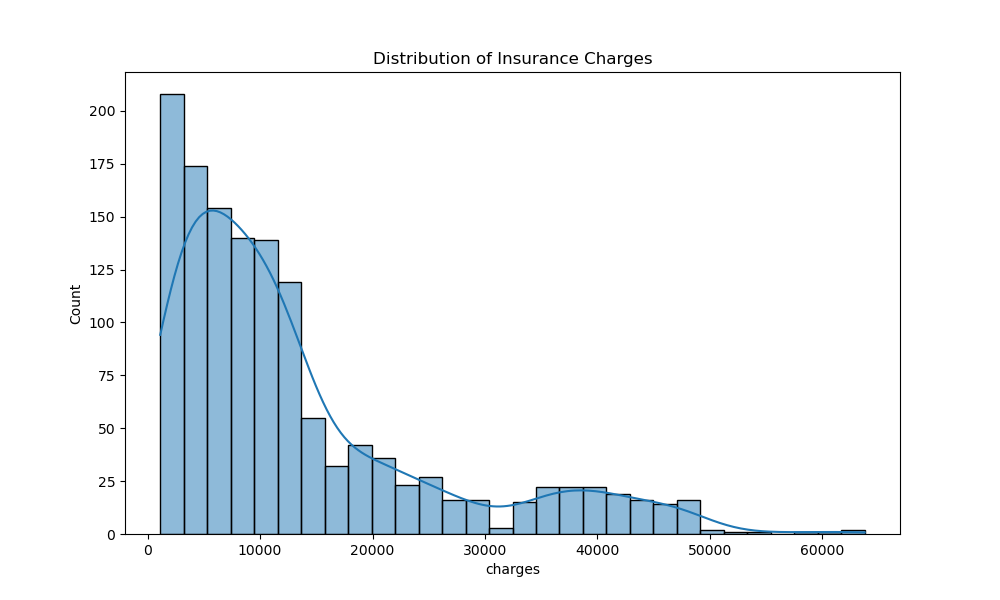
\includegraphics[width=0.8\textwidth]{charges_dist.png}
\caption{Distribution of Insurance Charges}
\end{figure}
\end{frame}

\begin{frame}{Exploratory Data Analysis (Cont.)}
\begin{figure}
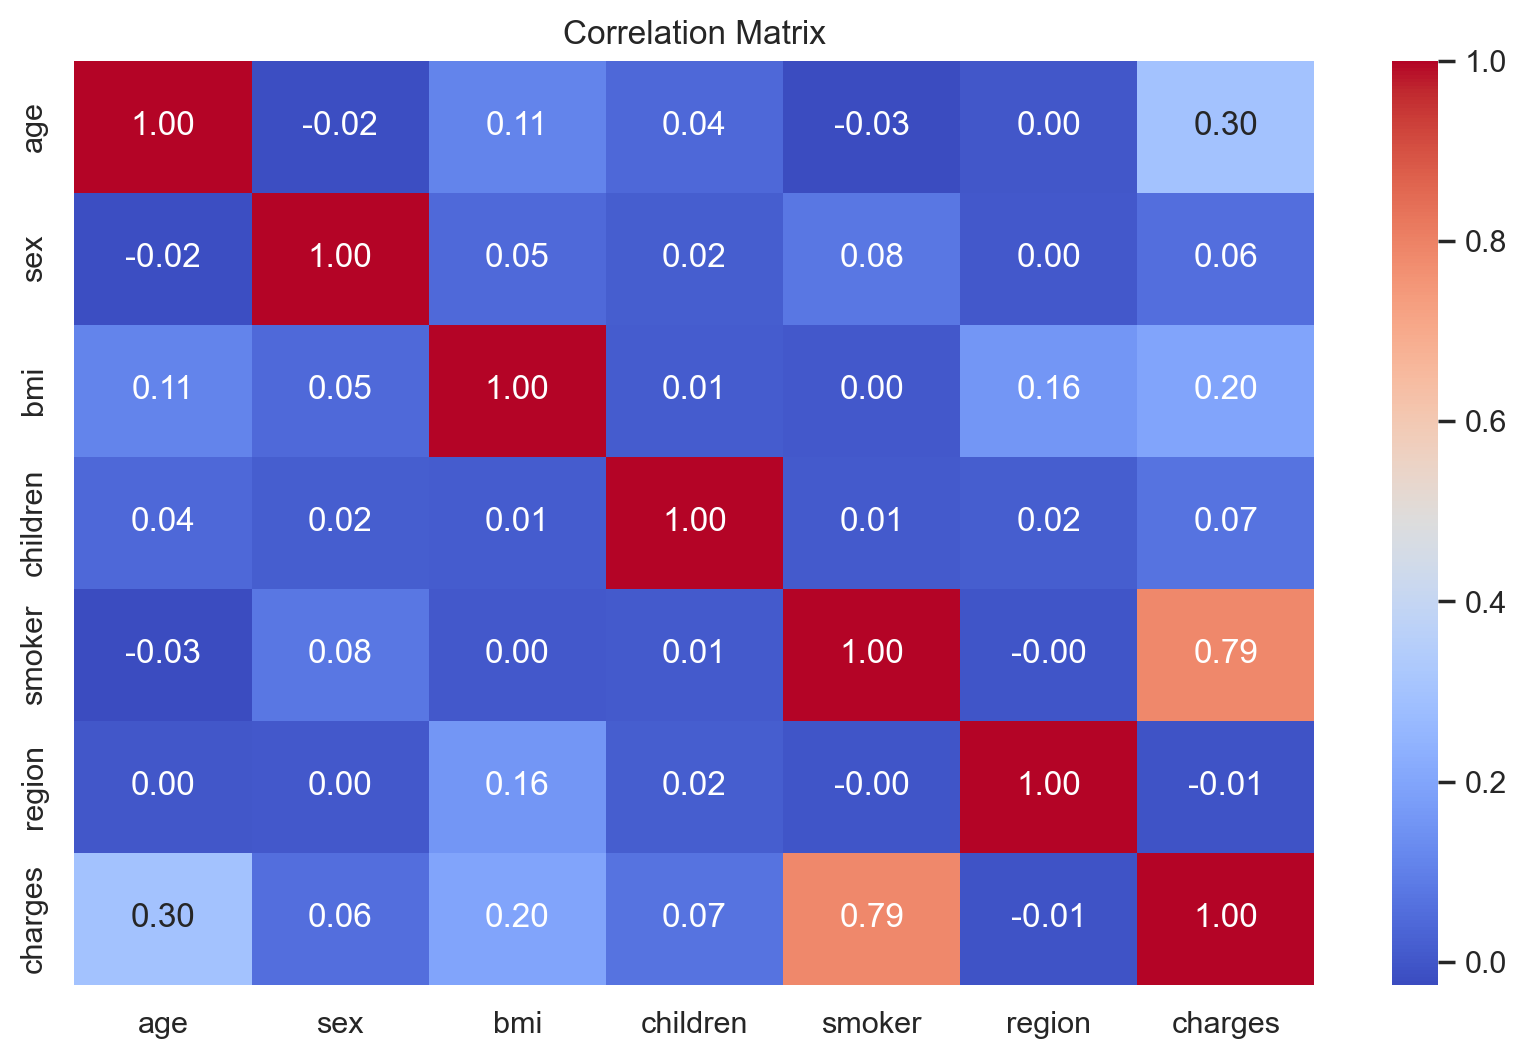
\includegraphics[width=0.8\textwidth]{correlation_heatmap.png}
\caption{Correlation Matrix}
\end{figure}
\begin{itemize}
\item Strong correlations: smoker (+0.79), age (+0.30), BMI (+0.20)
\item Regional variations in charges
\end{itemize}
\end{frame}

\begin{frame}{Preprocessing and Feature Engineering}
\begin{itemize}
  \item Label-encode: sex, smoker, region; derive bmi\_category and age\_group.
  \item Train/test split: 80/20 with fixed random seed for reproducibility.
  \item Standardize inputs with \texttt{StandardScaler} (fit on train, transform test).
  \item Keep target in original units (USD) to simplify interpretation of RMSE/MAE.
\end{itemize}
\end{frame}

\begin{frame}{Modeling Approach: Linear Regression}
\textbf{Ordinary Least Squares (OLS)}
\begin{itemize}
\item \textbf{Model}: $\hat{y} = \beta_0 + \sum_{j=1}^{p} \beta_j x_j$
\item \textbf{Objective}: Minimize sum of squared residuals
  $$\min_{\boldsymbol{\beta}} \sum_{i=1}^{n} (y_i - \hat{y}_i)^2 = \min_{\boldsymbol{\beta}} \|\mathbf{y} - \mathbf{X}\boldsymbol{\beta}\|^2$$
\item \textbf{Closed-form solution}: $\hat{\boldsymbol{\beta}} = (\mathbf{X}^T\mathbf{X})^{-1}\mathbf{X}^T\mathbf{y}$
\item \textbf{Assumptions}: Linearity, homoscedasticity, independence, normality
\item \textbf{Advantages}: Fast, interpretable coefficients, well-understood
\item \textbf{Limitations}: Cannot capture non-linear interactions (e.g., smoker × BMI)
\item \textbf{Test Performance}: R²=0.787, RMSE=\$5,747
\end{itemize}
\end{frame}

\begin{frame}{Modeling Approach: Decision Tree}
\textbf{Recursive Binary Partitioning}
\begin{itemize}
\item \textbf{Algorithm}: CART (Classification and Regression Trees)
\item \textbf{Splitting criterion}: Minimize variance at each node
  $$\text{MSE}_{\text{node}} = \frac{1}{n_{\text{node}}} \sum_{i \in \text{node}} (y_i - \bar{y}_{\text{node}})^2$$
\item \textbf{Feature selection}: Choose split that maximizes variance reduction
  $$\Delta = \text{MSE}_{\text{parent}} - \left(\frac{n_{\text{left}}}{n} \text{MSE}_{\text{left}} + \frac{n_{\text{right}}}{n} \text{MSE}_{\text{right}}\right)$$
\item \textbf{Advantages}: Non-linear, handles interactions, interpretable rules
\item \textbf{Limitations}: High variance (overfitting), unstable to data perturbations
\item \textbf{Test Performance}: R²=0.740, RMSE=\$6,354
\end{itemize}
\end{frame}

\begin{frame}{Modeling Approach: Random Forest}
\textbf{Bootstrap Aggregating (Bagging) of Decision Trees}
\begin{itemize}
\item \textbf{Ensemble method}: Train $B$ trees on bootstrap samples
  $$\hat{y}_{\text{RF}} = \frac{1}{B} \sum_{b=1}^{B} \hat{y}_b(\mathbf{x})$$
\item \textbf{Feature randomness}: At each split, consider random subset of $\sqrt{p}$ features
\item \textbf{Variance reduction}: Decorrelates trees, reduces overfitting
  $$\text{Var}(\bar{X}) = \frac{\sigma^2}{B} \quad \text{(for independent trees)}$$
\item \textbf{Out-of-bag (OOB) error}: Internal validation using ~37\% held-out samples
\item \textbf{Advantages}: Robust, handles high-dimensional data, reduces overfitting
\item \textbf{Baseline Performance}: R²=0.865, RMSE=\$4,574
\item \textbf{Optuna-tuned}: R²=0.879, RMSE=\$4,327 (+1.4\% improvement)
\end{itemize}
\end{frame}

\begin{frame}{Modeling Approach: XGBoost}
\textbf{Gradient Boosting with Regularization}
\begin{itemize}
\item \textbf{Additive model}: Build trees sequentially to correct residuals
  $$\hat{y}^{(t)} = \hat{y}^{(t-1)} + \eta \cdot f_t(\mathbf{x})$$
  where $\eta$ is the learning rate, $f_t$ is the $t$-th tree
\item \textbf{Objective function}: Loss + regularization
  $$\mathcal{L}^{(t)} = \sum_{i=1}^{n} \ell(y_i, \hat{y}_i^{(t)}) + \Omega(f_t)$$
  $$\Omega(f) = \gamma T + \frac{1}{2}\lambda \|\mathbf{w}\|^2 + \alpha \|\mathbf{w}\|_1$$
  ($T$ = \# leaves, $\mathbf{w}$ = leaf weights, $\gamma, \lambda, \alpha$ = regularization)
\item \textbf{Second-order approximation}: Uses gradient and Hessian for faster convergence
\item \textbf{Advantages}: State-of-the-art accuracy, handles missing data, parallelized
\item \textbf{Optuna-tuned Performance}: R²=0.879, RMSE=\$4,331
\end{itemize}
\end{frame}

\begin{frame}{Evaluation Metrics}
\textbf{Regression Performance Measures}
\begin{itemize}
\item \textbf{Coefficient of Determination (R²)}:
  $$R^2 = 1 - \frac{\sum_{i=1}^{n}(y_i - \hat{y}_i)^2}{\sum_{i=1}^{n}(y_i - \bar{y})^2} = 1 - \frac{\text{SS}_{\text{res}}}{\text{SS}_{\text{tot}}}$$
  Proportion of variance explained by the model (0 to 1, higher is better)
\item \textbf{Root Mean Squared Error (RMSE)}:
  $$\text{RMSE} = \sqrt{\frac{1}{n}\sum_{i=1}^{n}(y_i - \hat{y}_i)^2}$$
  Average prediction error in dollars (lower is better, sensitive to outliers)
\item \textbf{Mean Absolute Error (MAE)}:
  $$\text{MAE} = \frac{1}{n}\sum_{i=1}^{n}|y_i - \hat{y}_i|$$
  Median-like error metric (lower is better, robust to outliers)
\end{itemize}
\end{frame}

\begin{frame}{Validation and Evaluation}
\begin{itemize}
  \item Validation: 5-fold cross-validation on the training data to assess variance.
  \item Metrics reported: $R^2$, RMSE, MAE (on the holdout test set).
\end{itemize}
\vspace{4pt}
\small
\begin{table}[h]
\centering
\begin{tabular}{@{}lcc@{}}
\toprule
Model & Mean $R^2$ (5-fold) & Std \\
\midrule
Linear Regression & 0.738 & 0.049 \\
Decision Tree & 0.720 & 0.067 \\
Random Forest & 0.825 & 0.043 \\
\bottomrule
\end{tabular}
\caption{Cross-validation performance (training folds)}
\end{table}
\end{frame}

\begin{frame}{Hyperparameter Tuning with Optuna}
\begin{itemize}
  \item Bayesian optimization (TPE) over 20 trials per model to maximize $R^2$ on validation.
  \item Search spaces summarized below; priors encourage compact trees and regularization to reduce overfitting.
\end{itemize}
\small
\begin{table}[h]
\centering
\begin{tabular}{@{}lll@{}}
\toprule
Model & Hyperparameter & Range \\
\midrule
Random Forest & n\_estimators & 200--800 \\
Random Forest & max\_depth & 4--16 \\
Random Forest & min\_samples\_split & 2--20 \\
Random Forest & min\_samples\_leaf & 1--20 \\
XGBoost & n\_estimators & 200--800 \\
XGBoost & max\_depth & 3--8 \\
XGBoost & learning\_rate & 0.01--0.3 \\
XGBoost & subsample & 0.6--1.0 \\
XGBoost & colsample\_bytree & 0.6--1.0 \\
XGBoost & gamma & 0.0--5.0 \\
XGBoost & reg\_alpha, reg\_lambda & 0.0--10.0 \\
\bottomrule
\end{tabular}
\caption{Optuna search spaces}
\end{table}
\end{frame}

\begin{frame}{Best Hyperparameters Found}
\small
\begin{columns}
\begin{column}{0.48\textwidth}
\textbf{Random Forest}
\begin{table}[h]
\centering
\begin{tabular}{@{}ll@{}}
\toprule
Param & Value \\
\midrule
n\_estimators & 567 \\
max\_depth & 5 \\
min\_samples\_split & 7 \\
min\_samples\_leaf & 8 \\
\bottomrule
\end{tabular}
\end{table}
\end{column}
\begin{column}{0.52\textwidth}
\textbf{XGBoost}
\begin{table}[h]
\centering
\begin{tabular}{@{}ll@{}}
\toprule
Param & Value \\
\midrule
n\_estimators & 253 \\
max\_depth & 4 \\
learning\_rate & 0.0231 \\
subsample & 0.7301 \\
colsample\_bytree & 0.7555 \\
gamma & 1.3567 \\
reg\_alpha & 8.2874 \\
reg\_lambda & 3.5675 \\
\bottomrule
\end{tabular}
\end{table}
\end{column}
\end{columns}
\vspace{2pt}
Both tuned models achieve $R^2 \approx 0.879$ on the test set, improving over the untuned Random Forest.
\end{frame}

\begin{frame}{Key Findings \& Visualizations}
\begin{table}[h]
\centering
\small
\begin{tabular}{@{}lccc@{}}
\toprule
Model & R² & RMSE (\$) & MAE (\$) \\
\midrule
Linear Regression & 0.787 & 5,747 & 4,097 \\
Decision Tree & 0.740 & 6,354 & 2,878 \\
Random Forest (Baseline) & 0.865 & 4,574 & 2,503 \\
\textbf{Random Forest (Optuna)} & \textbf{0.879} & \textbf{4,327} & \textbf{2,458} \\
\textbf{XGBoost (Optuna)} & \textbf{0.879} & \textbf{4,331} & \textbf{2,479} \\
\bottomrule
\end{tabular}
\caption{Model Performance Comparison}
\end{table}
\begin{itemize}
\item \textbf{Best Model}: Tuned tree ensembles cluster at $R^2 \approx 0.879$ with $<\$4.35$k RMSE
\item \textbf{Improvement}: +1.4 $R^2$ points over the untuned Random Forest
\item Cross-validation confirms stability
\end{itemize}
\end{frame}

\begin{frame}{Model Performance: Visual Comparison}
\begin{figure}
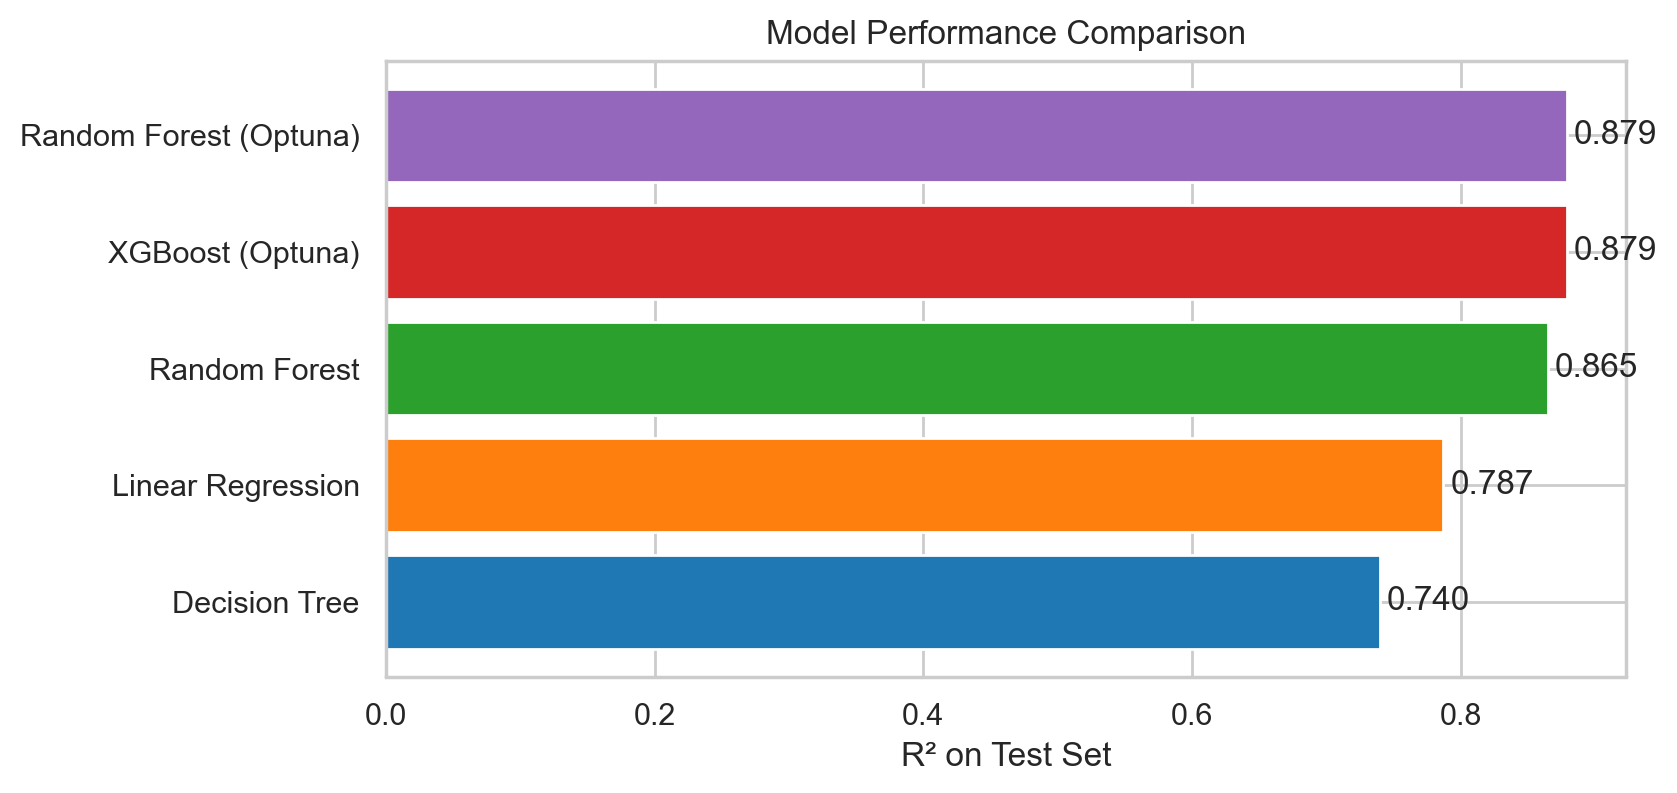
\includegraphics[width=0.9\textwidth]{model_comparison_all.png}
\caption{R$^2$ on test set across models (higher is better)}
\end{figure}
\end{frame}

\begin{frame}{Residual Diagnostics}
\begin{figure}
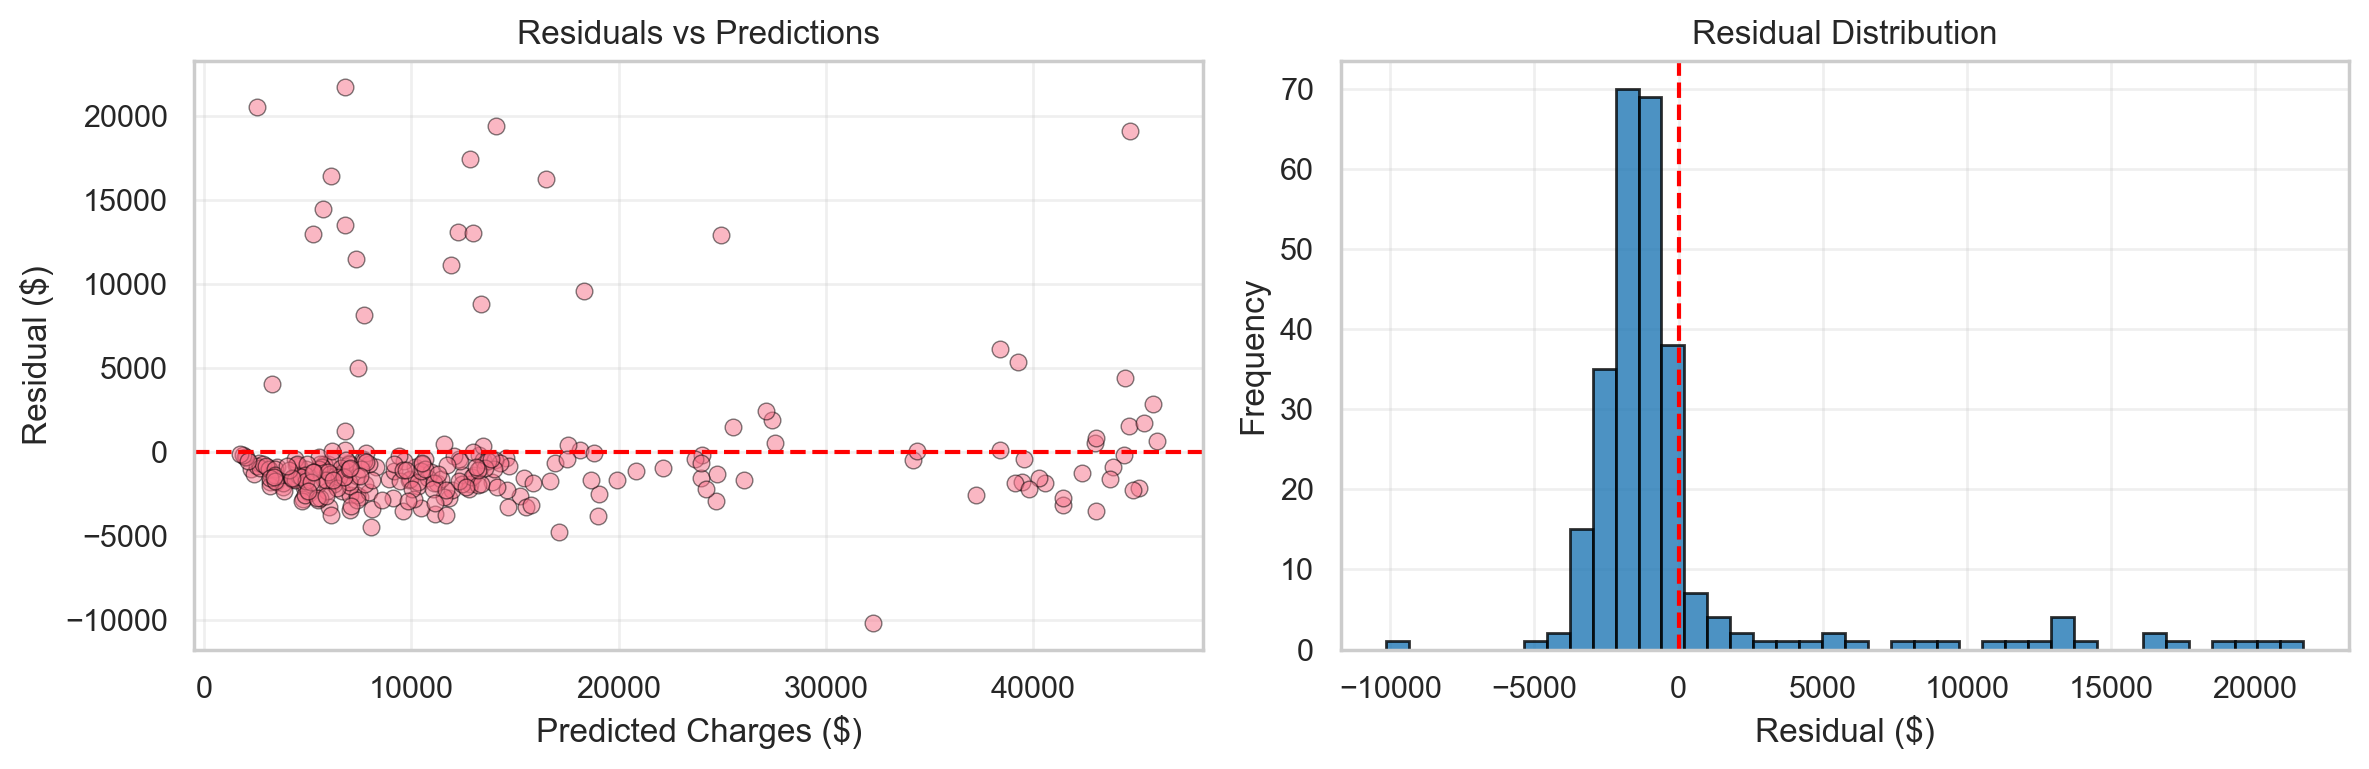
\includegraphics[width=0.92\textwidth]{residual_analysis.png}
\caption{Residuals vs predictions and residual distribution (tuned XGBoost)}
\end{figure}
\vspace{-6pt}
\small Mean residual $\approx -222$; standard deviation $\approx 4333$. Approximate symmetry and homoscedasticity are acceptable for pricing use cases.
\end{frame}

\begin{frame}{Permutation Importance (Random Forest)}
\begin{figure}
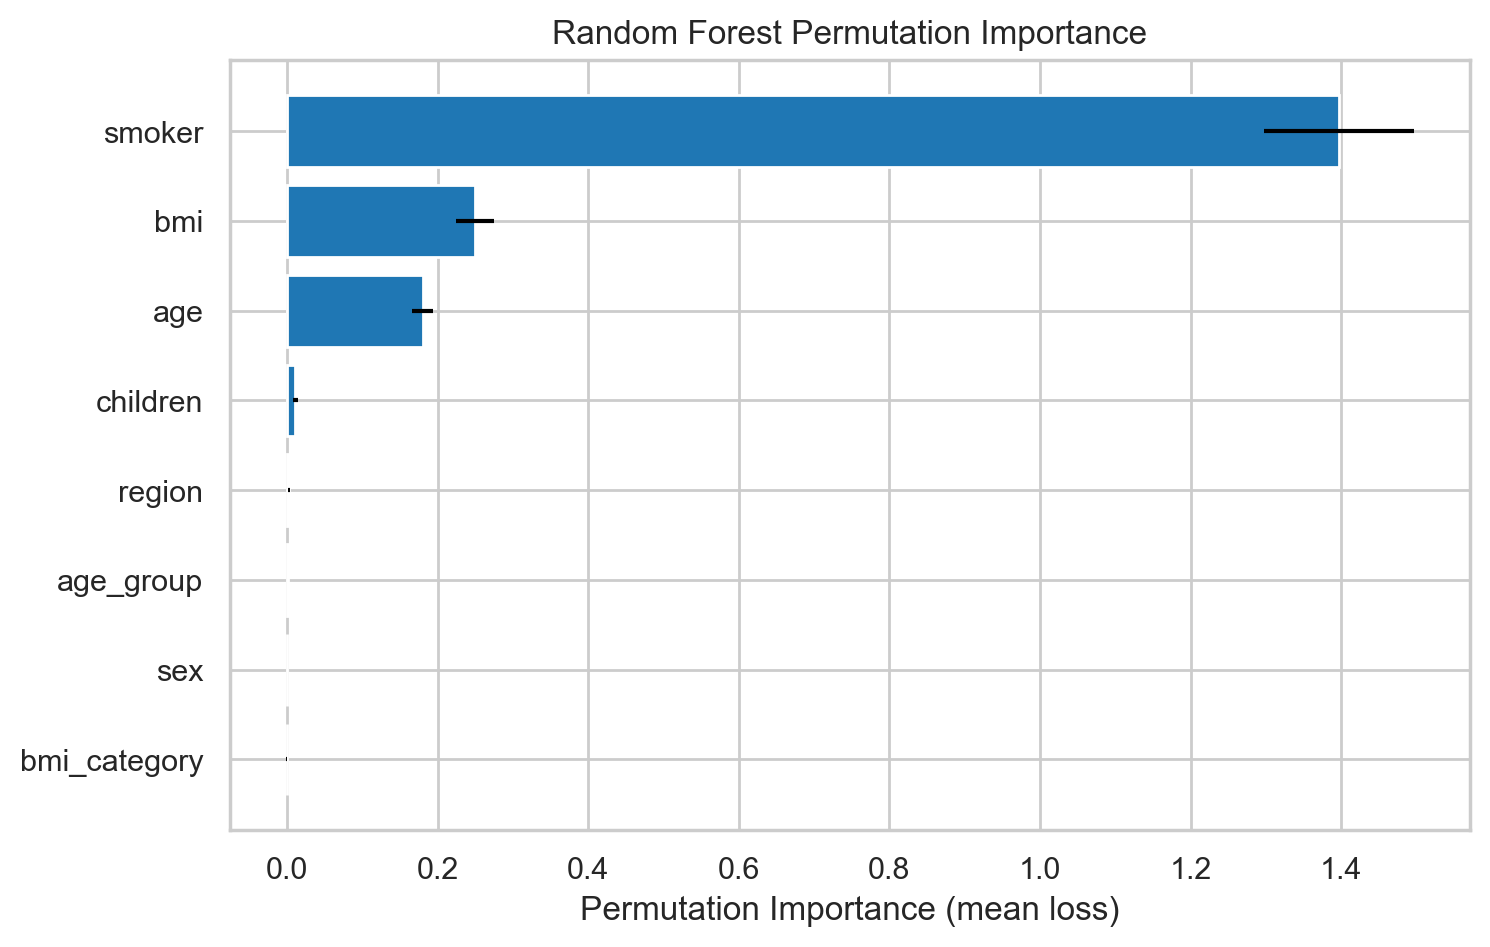
\includegraphics[width=0.9\textwidth]{feature_importance.png}
\caption{Permutation importance on the test split}
\end{figure}
\small Smoking, BMI, and Age dominate predictive power; this aligns with domain knowledge and SHAP analyses.
\end{frame}

\begin{frame}{Feature Impact Analysis}
\begin{columns}
\begin{column}{0.5\textwidth}
\begin{figure}
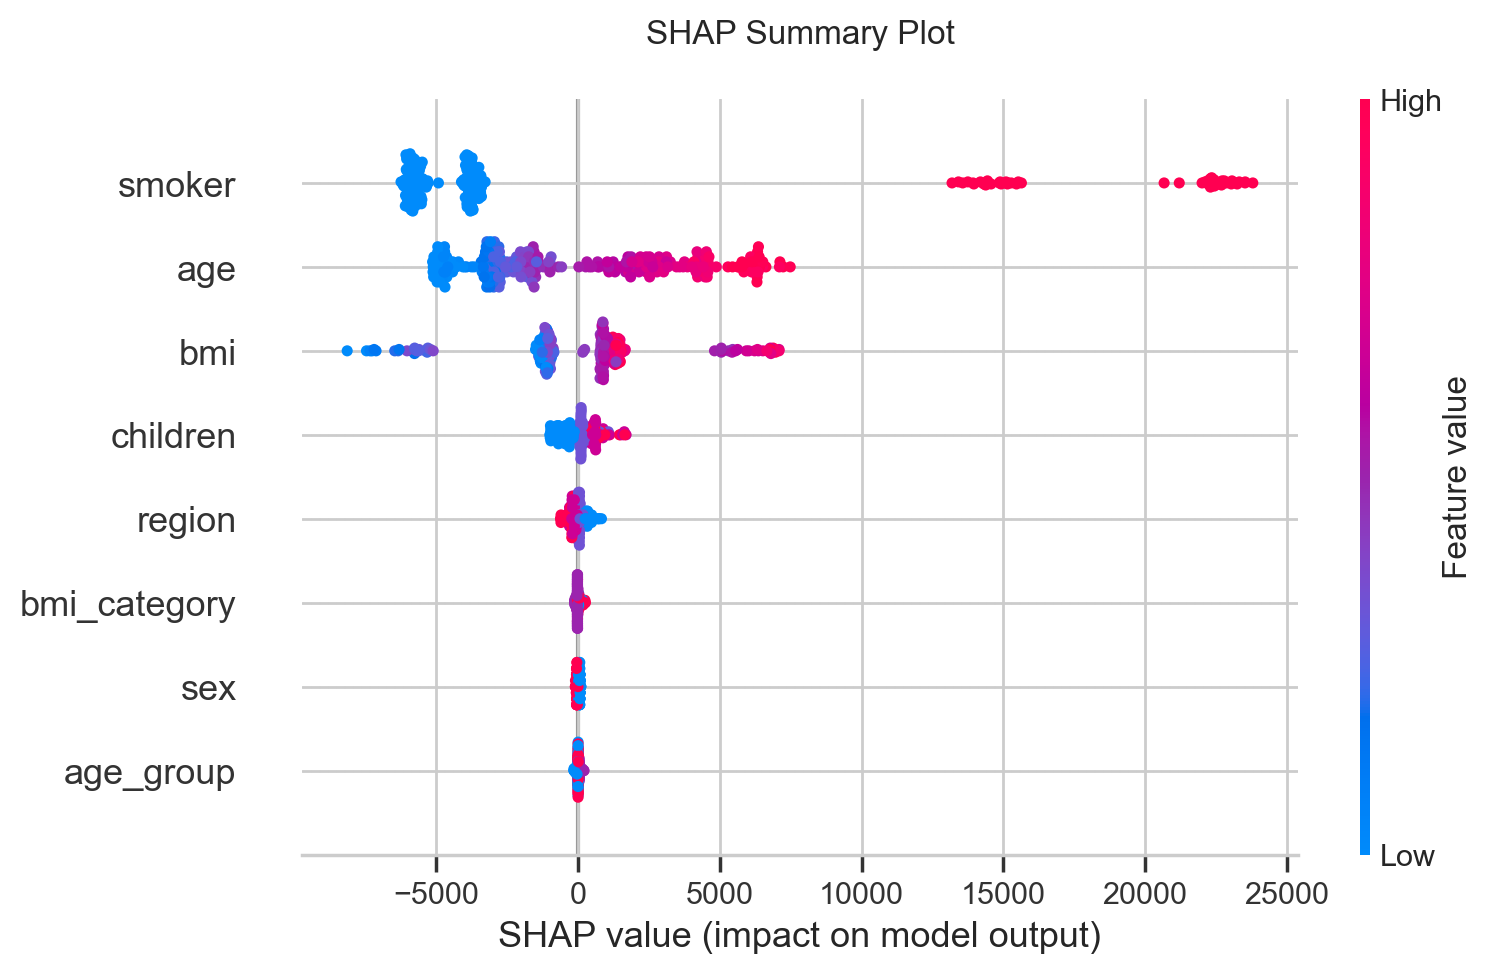
\includegraphics[width=\textwidth]{shap_summary.png}
\caption{SHAP Summary Plot}
\end{figure}
\end{column}
\begin{column}{0.5\textwidth}
\begin{figure}
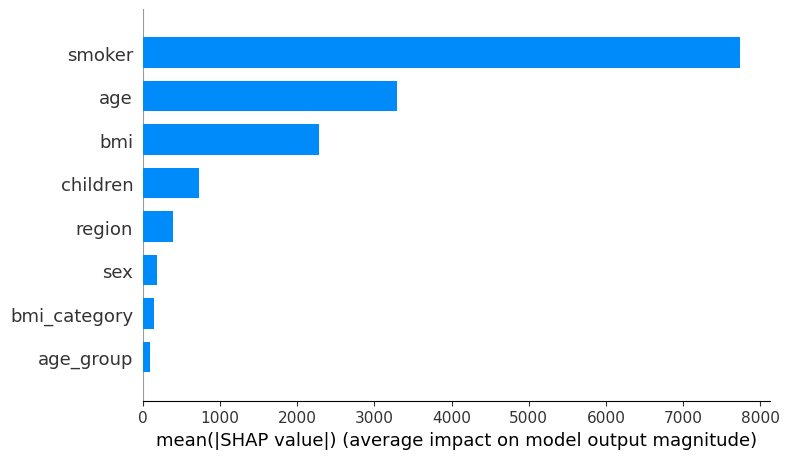
\includegraphics[width=\textwidth]{shap_bar.png}
\caption{SHAP Feature Importance}
\end{figure}
\end{column}
\end{columns}
\begin{itemize}
\item Top factors: Smoking (dominant), Age, BMI
\item Sex and region have minimal impact
\end{itemize}
\end{frame}

\begin{frame}{Partial Dependence Plots}
\begin{figure}
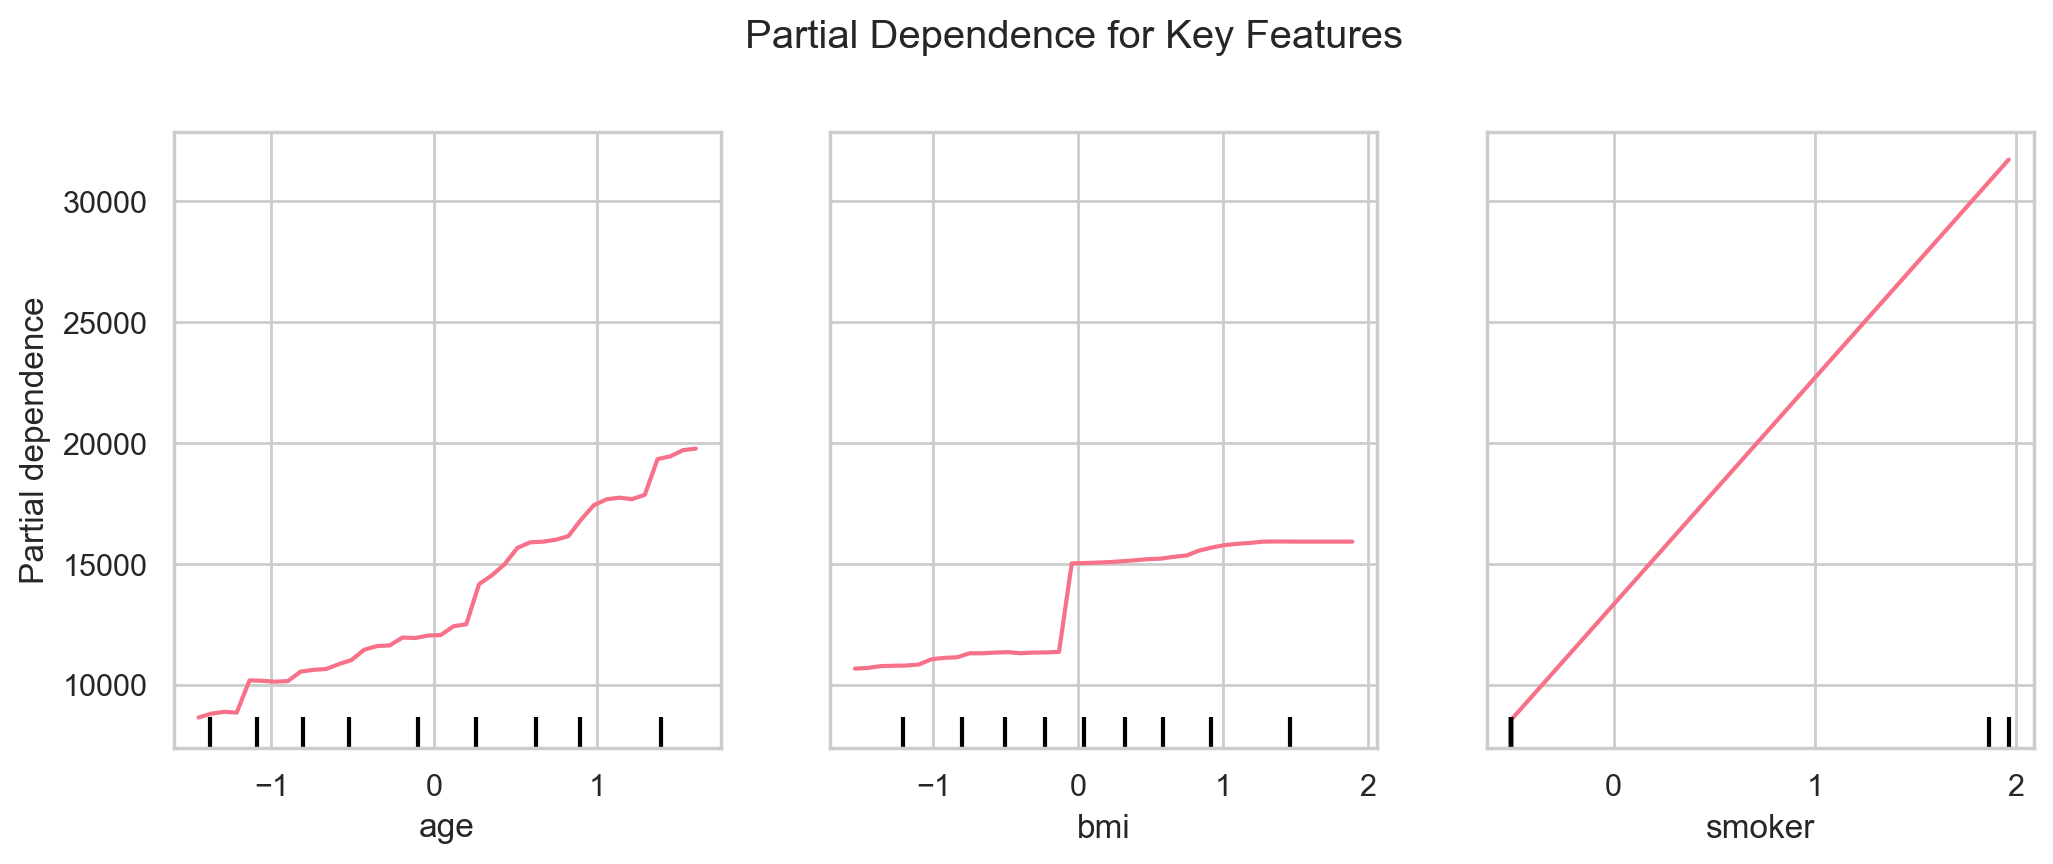
\includegraphics[width=0.95\textwidth]{pdp_core_features.png}
\caption{Marginal Effects of Key Features}
\end{figure}
\begin{itemize}
\item \textbf{Age}: Linear increase (\$8-10k from 20 to 60)
\item \textbf{BMI}: Gentle upward curve (accelerates above 30)
\item \textbf{Smoker}: Dramatic step function (+\$20k for smokers)
\end{itemize}
\end{frame}

\begin{frame}{Fairness Analysis}
\begin{columns}
\begin{column}{0.5\textwidth}
\begin{figure}
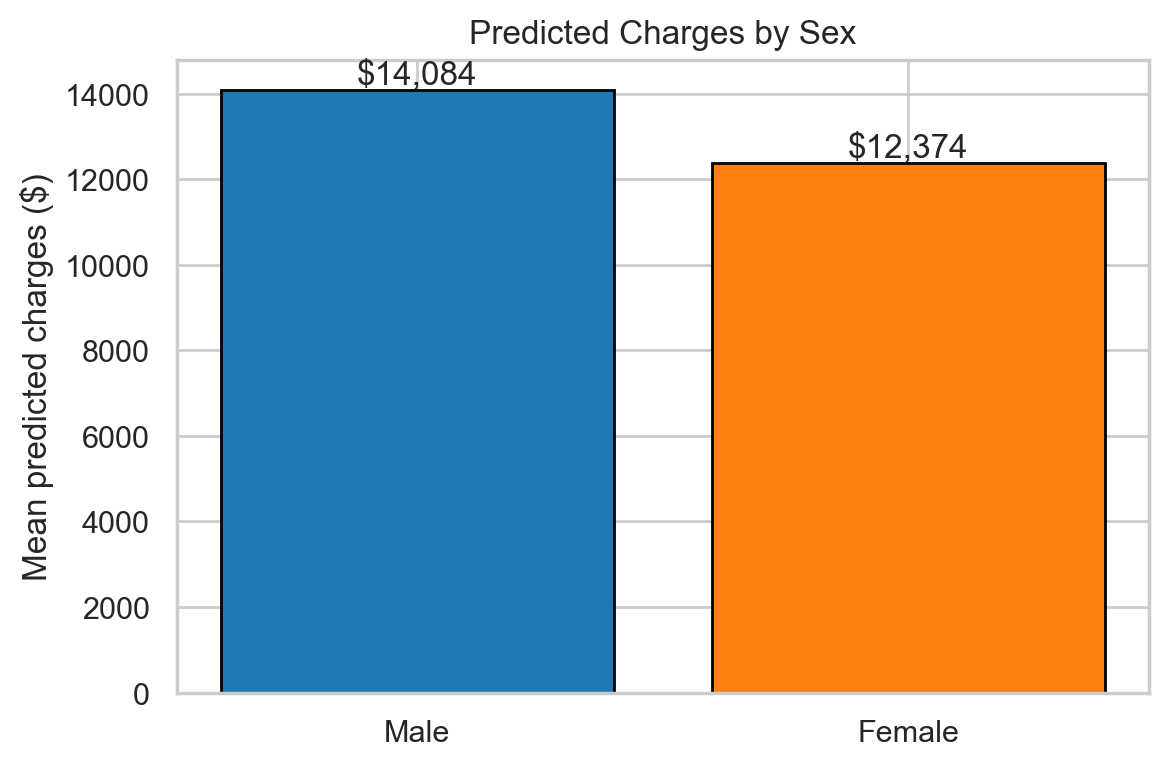
\includegraphics[width=\textwidth]{fairness_mean_pred_by_sex.png}
\caption{Charges by Sex}
\end{figure}
\end{column}
\begin{column}{0.5\textwidth}
\begin{figure}
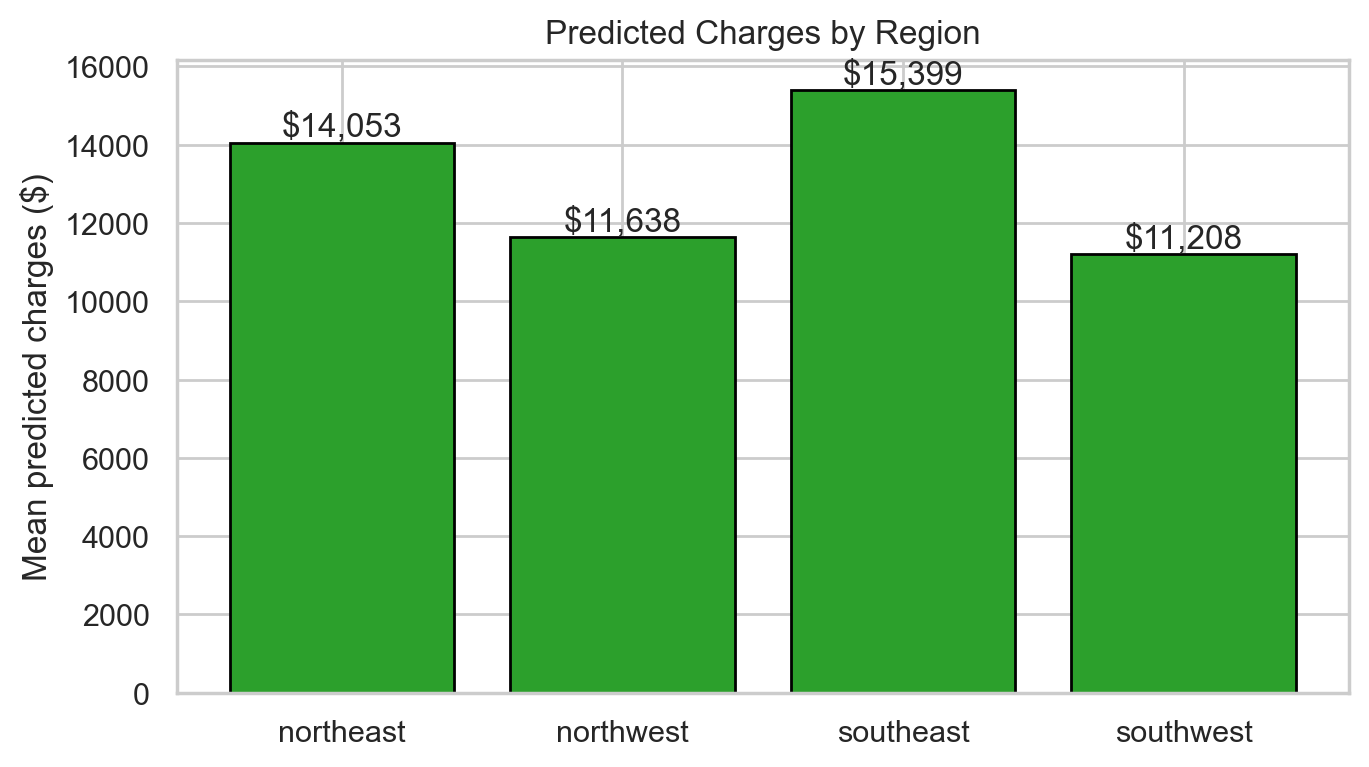
\includegraphics[width=\textwidth]{fairness_mean_pred_by_region.png}
\caption{Charges by Region}
\end{figure}
\end{column}
\end{columns}
\begin{itemize}
\item \textbf{Sex}: Welch's t-test p=0.226 $\rightarrow$ \textcolor{green}{\checkmark} No significant bias
\item \textbf{Region}: ANOVA p=0.091 $\rightarrow$ \textcolor{green}{\checkmark} Minimal bias
\item Differences reflect genuine risk factors, not discrimination
\end{itemize}
\end{frame}

\begin{frame}{Practical Recommendations}
\begin{itemize}
\item \textbf{For Insurers}:
  \begin{itemize}
  \item Deploy XGBoost with Optuna for premium calculation
  \item \textbf{Highest ROI}: Smoking cessation programs (\$20k impact)
  \item Target obesity prevention (BMI effect accelerates >30)
  \end{itemize}
\item \textbf{Policy Implications}:
  \begin{itemize}
  \item Fair pricing based on verifiable risks validated via statistical tests
  \item Monitor regional healthcare access disparities
  \item Implement quarterly fairness audits (NAIC recommendations)
  \end{itemize}
\item \textbf{Future Work}:
  \begin{itemize}
  \item Collect longitudinal data, medical history
  \item Disparate impact analysis (AI Fairness 360, Fairlearn)
  \item Avoid controversial proxies (credit scores, ZIP codes)
  \end{itemize}
\end{itemize}
\end{frame}

\begin{frame}{Difficulties Faced \& Solutions}
\begin{itemize}
\item \textbf{Dataset Limitations}:
  \begin{itemize}
  \item Small size (1,338 records) limits generalizability
  \item Missing features: medical history, genetics, lifestyle details
  \item Static data: no temporal health changes
  \end{itemize}
\item \textbf{Technical Challenges}:
  \begin{itemize}
  \item XGBoost version conflicts: Resolved via conda-forge channel
  \item SHAP API changes: Updated to new waterfall/summary plot syntax
  \item Model overfitting: Addressed with Optuna's Bayesian optimization
  \item PDP compatibility: Ensured fitted estimator passed correctly
  \end{itemize}
\item \textbf{Solutions}:
  \begin{itemize}
  \item Feature engineering for better segmentation
  \item Rigorous validation and error analysis
  \item Innovative explainability techniques
  \end{itemize}
\end{itemize}
\end{frame}

\begin{frame}{Conclusion}
\begin{itemize}
\item Successfully predicted \textbf{87.9\%} of insurance cost variance (tuned ensembles)
\item Smoking is the dominant factor (+\$20k), followed by age and BMI
\item Models validated as fair through statistical testing (p>0.05)
\item Full interpretability via SHAP and PDPs ensures transparency
\item Future: Larger datasets, disparate impact analysis, advanced AI
\end{itemize}
\begin{center}
\textbf{Thank you for your attention!}
\end{center}
\end{frame}

\end{document}
